\documentclass[11pt,a4paper]{article}

\usepackage[T1]{fontenc}
\usepackage[english]{babel}
\usepackage[a4paper,margin=2.5cm]{geometry}
\usepackage{array}
\usepackage{float}
\usepackage{graphicx}
\usepackage{hyperref}
\usepackage[table]{xcolor}
\usepackage{tikz}

\hypersetup{hidelinks}
\renewcommand{\contentsname}{Index}
\setcounter{tocdepth}{1}
\setcounter{secnumdepth}{0}
\setlength{\parindent}{0pt}
\setlength{\parskip}{0.6em}

% Shared starter report.
% This file contains a partial set of sample findings and evidence notes.
% It is meant to help structure a report, not to replace an audit.

\newcommand{\reportfigure}[2]{%
  \begin{figure}[H]
    \centering
    \IfFileExists{#1}{%
      \includegraphics[width=0.82\textwidth]{#1}%
    }{%
      \fcolorbox{PanelBorder}{gray!8}{%
        \parbox{0.82\textwidth}{%
          \centering
          Screenshot placeholder\\[0.4em]
          Expected file:\\
          \path{#1}%
        }%
      }%
    }%
    \caption{#2}
  \end{figure}
}

\newcommand{\cvsstable}[8]{%
  \begin{center}
    \begin{tabular}{|>{\centering\arraybackslash}m{0.85cm}|>{\centering\arraybackslash}m{0.85cm}|>{\centering\arraybackslash}m{0.85cm}|>{\centering\arraybackslash}m{0.85cm}|>{\centering\arraybackslash}m{0.85cm}|>{\centering\arraybackslash}m{0.85cm}|>{\centering\arraybackslash}m{0.85cm}|>{\centering\arraybackslash}m{0.85cm}|}
      \hline
      AV & AC & PR & UI & S & C & I & A \\
      \hline
      #1 & #2 & #3 & #4 & #5 & #6 & #7 & #8 \\
      \hline
    \end{tabular}
  \end{center}
}

\newcommand{\riskchartstarter}{%
  \begin{center}
    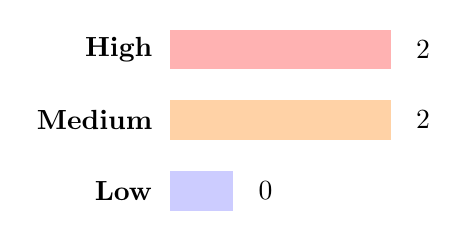
\begin{tikzpicture}[x=1cm,y=1cm]
      \fill[red!30] (0,1.8) rectangle (2.8,2.3);
      \fill[orange!35] (0,0.9) rectangle (2.8,1.4);
      \fill[blue!20] (0,0.0) rectangle (0.8,0.5);

      \node[anchor=east] at (-0.1,2.05) {\textbf{High}};
      \node[anchor=east] at (-0.1,1.15) {\textbf{Medium}};
      \node[anchor=east] at (-0.1,0.25) {\textbf{Low}};

      \node[anchor=west] at (3.0,2.05) {2};
      \node[anchor=west] at (3.0,1.15) {2};
      \node[anchor=west] at (1.0,0.25) {0};
    \end{tikzpicture}
  \end{center}
}

\begin{document}

\pagenumbering{gobble}
\begin{titlepage}
  \centering
  \vspace*{1cm}
  \IfFileExists{../others/Epita.jpg}{
\includegraphics[width=0.22\textwidth]{../others/Epita.jpg}\par}{}
  \vspace{1.5cm}

  {\Huge Security Assessment Report\par}
  \vspace{0.3cm}
  {\Large StockApp\par}
  \vspace{1cm}
  {\large Software and Database Security\par}

  \vfill

  \begin{tabular}{rl}
    Group: & Masters of Computer Science, Software Engineering \\
    Class of: & Fall 2025 \\
    Prepared on: & 5 April 2026 \\
    Authors: & Example Group \\
  \end{tabular}

  \vfill

  {\large EPITA\par}
\end{titlepage}

\pagenumbering{roman}
\tableofcontents
\clearpage
\pagenumbering{arabic}

\section{Synthesis}

This report presents the results of a security assessment performed on StockApp. The review focused on authentication, input handling, command execution, and local secret storage. This starter version includes four sample findings in order to provide a usable structure for the final report while leaving room for additional vulnerabilities, screenshots, and customer-specific details.

Two of the retained findings are high risk because they allow user-controlled input to alter backend behavior in a way that can disclose sensitive information or execute unintended commands. The remaining two findings are medium risk because they weaken the protection of credentials and authentication workflows. Even where exploitation requires local access or valid credentials, the resulting exposure remains significant because the application handles account data and interacts with a database.

Priority remediation should focus on removing unsafe SQL and command construction first. After those issues are addressed, secrets should no longer be stored in plaintext configuration files and the login process should be protected against repeated guessing attempts. The final version of the report can extend this synthesis with the full number of findings, exact risk distribution, and any business-specific impact observed during the audit.

\begin{center}
  \begin{tabular}{|l|c|}
    \hline
    Risk level & Number of findings \\
    \hline
    High & 2 \\
    \hline
    Medium & 2 \\
    \hline
    Low & 0 \\
    \hline
  \end{tabular}
\end{center}

\riskchartstarter

\clearpage
\section{SQL Injection}

\textbf{Common Weakness Enumeration (CWE) ID}\\
\href{https://cwe.mitre.org/data/definitions/89.html}{CWE-89: Improper Neutralization of Special Elements used in an SQL Command ('SQL Injection')}

\subsection*{CVSS 3.1 Base Score Metrics}
\textbf{Vector:} \href{https://nvd.nist.gov/vuln-metrics/cvss/v3-calculator?vector=AV:L/AC:L/PR:L/UI:N/S:U/C:H/I:H/A:N&version=3.1}{AV:L/AC:L/PR:L/UI:N/S:U/C:H/I:H/A:N}\\
\textbf{Score:} 7.1\\
\textbf{Risk level:} High

\cvsstable{L}{L}{L}{N}{U}{H}{H}{N}

\subsection*{Description}
The application builds a SQL query with user-controlled input instead of separating code from data. A user who reaches the vulnerable search feature can modify the query and retrieve records that should not be exposed. The business impact is unauthorized disclosure of account information and loss of trust in the integrity of the application data.

\subsection*{Exploitation}
The vulnerable feature is reached after a normal login to the application.

\reportfigure{../screenshots/cwe-89-step-1.png}{Application menu displayed after a successful login, showing that the article search feature is reachable by a standard user.}

Once the search field is available, a crafted payload is entered in place of a normal article name. A payload such as \texttt{" UNION SELECT username, password, NULL FROM users; -- } can force the application to return credential data from the users table.

\reportfigure{../screenshots/cwe-89-step-2.png}{Injected SQL payload entered in the article-name field, followed by the returned result containing rows that should not be disclosed.}

If usernames and passwords are displayed in the result set, the query has been altered successfully and the vulnerability is confirmed.

\subsection*{Remediation}
All database interactions should use parameterized queries or prepared statements. Input validation should reject unexpected values before they reach the SQL layer, and the database account used by the application should be restricted to the minimum privileges required by the feature. Reference: \href{https://cheatsheetseries.owasp.org/cheatsheets/SQL_Injection_Prevention_Cheat_Sheet.html}{OWASP SQL Injection Prevention Cheat Sheet}.

\clearpage
\section{Command Injection via Ping}

\textbf{Common Weakness Enumeration (CWE) ID}\\
\href{https://cwe.mitre.org/data/definitions/78.html}{CWE-78: Improper Neutralization of Special Elements used in an OS Command ('OS Command Injection')}

\subsection*{CVSS 3.1 Base Score Metrics}
\textbf{Vector:} \href{https://nvd.nist.gov/vuln-metrics/cvss/v3-calculator?vector=AV:L/AC:L/PR:L/UI:N/S:U/C:H/I:H/A:H&version=3.1}{AV:L/AC:L/PR:L/UI:N/S:U/C:H/I:H/A:H}\\
\textbf{Score:} 7.8\\
\textbf{Risk level:} High

\cvsstable{L}{L}{L}{N}{U}{H}{H}{H}

\subsection*{Description}
The connectivity test passes user input to an operating system command without safely neutralizing shell metacharacters. A user can therefore append additional commands and execute them in the context of the application. This can expose host-level information or allow unintended actions on the local machine.

\subsection*{Exploitation}
The connectivity option is opened from the application menu.

\reportfigure{../screenshots/cwe-078-step-1.png}{Connectivity-check screen or console prompt before the host value is entered.}

Instead of a normal IP address or hostname, the user enters a chained value such as \texttt{127.0.0.1 \&\& net user}. If the application interprets the second command and prints its output, the ping feature is vulnerable to command injection.

\reportfigure{../screenshots/cwe-078-step-2.png}{Chained command entered into the host field and the resulting system output produced by the injected command.}

The presence of local command output confirms that the application is executing shell content that should have been treated as plain input.

\subsection*{Remediation}
The feature should avoid shell execution entirely. If a system call remains necessary, the application must pass the destination as a single validated argument without invoking a command interpreter. The host field should be allowlisted, and the process should run with minimal privileges. Reference: \href{https://cheatsheetseries.owasp.org/cheatsheets/OS_Command_Injection_Defense_Cheat_Sheet.html}{OWASP OS Command Injection Defense Cheat Sheet}.

\clearpage
\section{Plaintext Credentials in \texttt{config.ini}}

\textbf{Common Weakness Enumeration (CWE) ID}\\
\href{https://cwe.mitre.org/data/definitions/312.html}{CWE-312: Cleartext Storage of Sensitive Information}

\subsection*{CVSS 3.1 Base Score Metrics}
\textbf{Vector:} \href{https://nvd.nist.gov/vuln-metrics/cvss/v3-calculator?vector=AV:L/AC:L/PR:N/UI:N/S:U/C:H/I:L/A:N&version=3.1}{AV:L/AC:L/PR:N/UI:N/S:U/C:H/I:L/A:N}\\
\textbf{Score:} 6.4\\
\textbf{Risk level:} Medium

\cvsstable{L}{L}{N}{N}{U}{H}{L}{N}

\subsection*{Description}
The application stores sensitive credentials in a local configuration file in plaintext form. Any user with access to the installation directory can read these values and reuse them directly against the associated service. The business impact is exposure of backend access outside the intended application workflow.

\subsection*{Exploitation}
The application configuration file is opened from the local installation directory.

\reportfigure{../screenshots/cwe-312.png}{Configuration file opened locally, with database credentials or other sensitive values visible in plaintext.}

If usernames, passwords, or connection strings are visible without encryption or further protection, the weakness is confirmed. These values can then be reused directly by an attacker.

\subsection*{Remediation}
Sensitive credentials should be removed from flat configuration files and moved to a protected secret store provided by the operating system or deployment environment. Existing secrets should be rotated and file permissions should be reduced to the minimum account that requires access. Reference: \href{https://cheatsheetseries.owasp.org/cheatsheets/Secrets_Management_Cheat_Sheet.html}{OWASP Secrets Management Cheat Sheet}.

\clearpage
\section{No Brute Force Protection}

\textbf{Common Weakness Enumeration (CWE) ID}\\
\href{https://cwe.mitre.org/data/definitions/307.html}{CWE-307: Improper Restriction of Excessive Authentication Attempts}

\subsection*{CVSS 3.1 Base Score Metrics}
\textbf{Vector:} \href{https://nvd.nist.gov/vuln-metrics/cvss/v3-calculator?vector=AV:L/AC:L/PR:N/UI:N/S:U/C:L/I:L/A:N&version=3.1}{AV:L/AC:L/PR:N/UI:N/S:U/C:L/I:L/A:N}\\
\textbf{Score:} 5.3\\
\textbf{Risk level:} Medium

\cvsstable{L}{L}{N}{N}{U}{L}{L}{N}

\subsection*{Description}
The authentication workflow accepts repeated password attempts without lockout, throttling, or meaningful delay. This lowers the cost of password guessing and makes automated attacks practical against weak or reused credentials.

\subsection*{Exploitation}
The same account is tested repeatedly with invalid passwords through the login prompt.

\reportfigure{../screenshots/cwe-307.png}{Repeated failed login attempts for the same account, with no lockout or delay applied between attempts.}

If the application continues to accept new attempts immediately and does not introduce a lockout, delay, or challenge step, the absence of brute force protection is confirmed.

\subsection*{Remediation}
Authentication attempts should be rate-limited and logged. After a defined number of failures, the application should apply progressive delays, lockout controls, or an additional verification step. Strong password policy enforcement should complement these controls. Reference: \href{https://cheatsheetseries.owasp.org/cheatsheets/Authentication_Cheat_Sheet.html}{OWASP Authentication Cheat Sheet}.

% Add further findings by copying one complete section block.

\end{document}
